%!TEX root = main.tex
%=================TD functions==================
\def\boldcommandlist{\@elt OP,\@elt OPs,}
\def\@elt#1,{%
 \expandafter\def\csname#1\endcsname{\textbf{#1}\xspace}
}
\boldcommandlist

\def\topColorList{\@elt TOP,\@elt TOPs,}
\def\@elt#1,{%
 \expandafter\def\csname#1\endcsname{\textcolor{TOP}{\textbf{#1}}\xspace}
}
\topColorList

\def\chopColorList{\@elt CHOP,\@elt CHOPs,}
\def\@elt#1,{%
 \expandafter\def\csname#1\endcsname{\textcolor{CHOP}{\textbf{#1}}\xspace}
}
\chopColorList

\def\sopColorList{\@elt SOP,\@elt SOPs,}
\def\@elt#1,{%
 \expandafter\def\csname#1\endcsname{\textcolor{SOP}{\textbf{#1}}\xspace}
}
\sopColorList

\def\datColorList{\@elt DAT,\@elt DATs,}
\def\@elt#1,{%
 \expandafter\def\csname#1\endcsname{\textcolor{DAT}{\textbf{#1}}\xspace}
}
\datColorList

\def\matColorList{\@elt MAT,\@elt MATs,}
\def\@elt#1,{%
 \expandafter\def\csname#1\endcsname{\textcolor{MAT}{\textbf{#1}}\xspace}
}
\matColorList


\def\compColorList{\@elt COMP,\@elt COMPs,}
\def\@elt#1,{%
 \expandafter\def\csname#1\endcsname{\textcolor{COMP}{\textbf{#1}}\xspace}
}
\compColorList

\def\redcommandlist{\@elt missingImage,}
\def\@elt#1,{%
 \expandafter\def\csname#1\endcsname{\textcolor{red}{\textbf{#1}}\xspace}
}
\redcommandlist

%===============================================

\chapter{Lecture 4}

\section{Notes}

\begin{itemize}
	\item more proc modeling
	\item parent shortcuts
	\item custom parameters
	\item modules
	\item structured work
	\item Cloning
	\item Replicator
	\item ui building
\end{itemize}

\section{Project Setup and Structure}

There are a lot of ways to set up a project for live performance. Different projects will require different structures and setups. Here, we will have a look at one suggestion. This suggestion is designed to fulfill the following criteria:
\begin{itemize}
	\item Being non-Linear and interactive
	\item Being somewhat tidy
	\item having multiple scenes
	\item having multiple FX
	\item each scene can be combined with each Effect
	\item Having a GUI
	\item each scene can react to audio without the need to duplicate the audio analysis
	\item versatile Output
	\item Minimize time for on-site configurations and adaptions
\end{itemize}


The project will be set up in a hierarchical way. In \texttt{root} we find a structure that looks like Figure \ref{fig:projectSchematic}.

	\begin{figure}[H]
	\centering


	% \resizebox{10cm}{!}{%
	\begin{tikzpicture}[auto, thick, node distance=2.3cm, >=triangle 45]

	\draw node at (5,0) [block] (audio) {$Audio$};
	\draw node [block, right of=audio, node distance = 2cm] (core) {$Core$};
	\draw node [block, right of=core, node distance = 2cm] (post) {$Post$};
	\draw node [block, right of=post, node distance = 2cm] (mapping) {$mapping$};
	\draw node [block, right of=mapping, node distance = 2cm] (output) {$output$};
	\draw node [block, below of=output, node distance = 2cm] (local) {$local$};
	\draw node [block, above of=audio, node distance = 2cm] (hid) {$midi$};
	\draw node [block, above of=core, node distance = 2cm] (ui) {$ui$};

  \draw[->] (hid) -- node {}(ui);
  \draw[->] (ui) -- node {}(core);
  \draw[->] (audio) -- node {}(core);
  \draw[->] (core) -- node {}(post);
  \draw[->] (post) -- node {}(mapping);
  \draw[->] (ui) -| node {}(output);
    \draw[->] (mapping) -- node {}(output);

  \end{tikzpicture}
  \caption{Schematic view of our project}
  \label{fig:projectSchematic}
\end{figure}

In practice, this might look like in Figure \ref{fig:structPraxis}.
\begin{figure}[H]
	\centering
	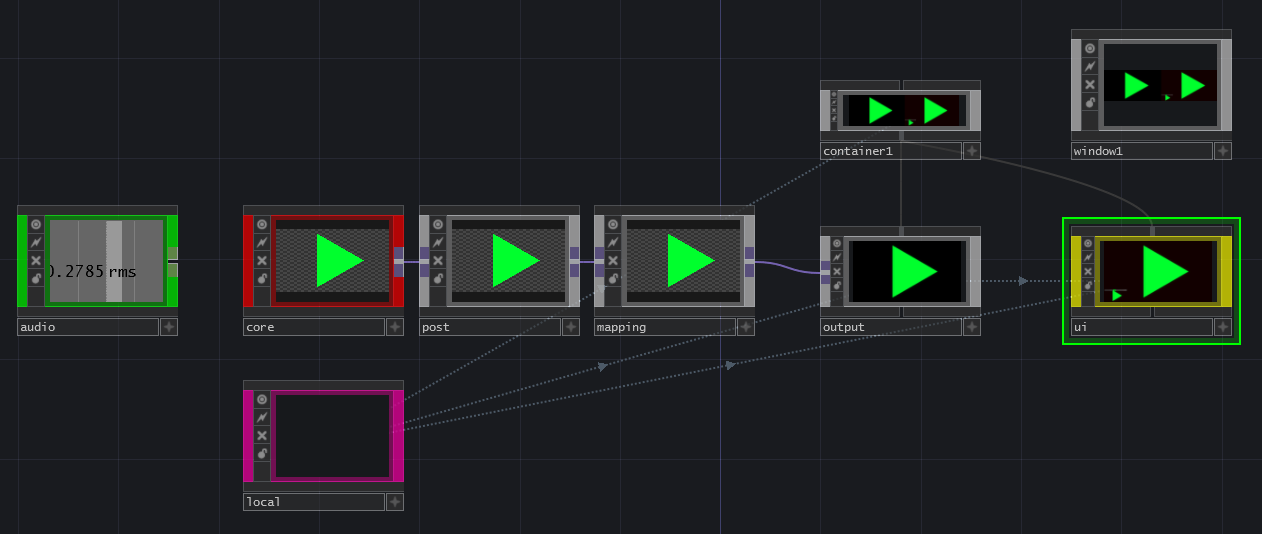
\includegraphics[width=\textwidth]{img/structure1.PNG}
	\caption[shortCaption]
	{Root level of our Project, inside \texttt{/project1/}}
	\label{fig:structPraxis}
\end{figure}

Notice that some arrows exist in the schematic but don't have corresponding patch cords in Figure \ref{fig:structPraxis}. This is because the information is flowing via references and/or Select \OPs.

Let's now have a look at what happens in each of these \COMPs.

\paragraph*{Midi}
We could also name this 'HID'(Human Interface devices). This could manage OSC\footnote{Open Sound control, a very common protocol for inter device communication typically running on top of the UDP protocol}. Typically some form of hardware device is used to control elements on the UI which then control the actual parameters.
\paragraph*{UI}
The UI Component is typically a Container \COMP. It holds the Graphical User Interface we see during our Show. It contains Sliders and other controls, previews of currently unused scenes and shows us our actual output in case we don't see our projection. It should also show us some information about audio input levels (This is not shown in figure \ref{fig:projectSchematic}).
Also it is used by the output, since we typically create one window spanning over all our monitors.\\
The UI can instantiate other UIs and can hold stored data.
\paragraph*{Audio}
Here we find our audio input (Audio Device In \CHOP) and all the audio analysis. The analyzed values (e.g. the current RMS) is then used by scenes in \texttt{core}.
\paragraph*{Core}
Here we actually create our different scenes and effects.
A very typical setup inside \texttt{core} could look like Figure \ref{fig:coreSchematic}. This is only one possibly topology of our image generation. We could also create our show using just one versatile algorithm with many parameters and possibly preset store/load facilities or we could go for a more interconnected matrix-like layout.


\begin{figure}[H]
	\centering

	\begin{tikzpicture}[auto, thick, node distance=2.3cm, >=triangle 45]

	\draw node at (5,0) [block] (scene1) {$scene\ 1$};
	\draw node [block, below of=scene1, node distance = 2cm] (scene2) {$scene\ 2$};
	\draw node [block, below of=scene2, node distance = 2cm] (scene3) {$scene\ 3$};

	\draw node [block, right of=scene1, node distance = 3cm] (switch1) {$switch$};
	\draw node [block, right of=switch1, node distance = 3cm] (fx1) {$fx\ 1$};
	\draw node [block, below of=fx1, node distance = 2cm] (fx2) {$fx\ 2$};
	\draw node [block, below of=fx2, node distance = 2cm] (fx3) {$fx\ 3$};

	\draw node [block, right of=fx1, node distance = 3cm] (switch2) {$switch$};

	\draw node [block, right of=switch2, node distance = 3cm] (output) {$output$};

	\foreach \point in {(5,-5.2),(5,-5.8),(5,-6.3)}{% points
    \fill \point circle (1pt);
}
\foreach \point in {(11,-5.2),(11,-5.8),(11,-6.3)}{% points
    \fill \point circle (1pt);
}



	\draw  node [right of=scene1, node distance = 1.5cm] (bp){};
	\draw  node [right of=switch1, node distance = 1.5cm] (bp2){};
	\draw  node [right of=fx1, node distance = 1.5cm] (bp3){};

	\draw[->] (scene1.east) -- node {}(switch1);
	\draw[->] (scene2.east) -| node{}(bp) -- node {}(switch1);
	\draw[->] (scene3.east) -| node{}(bp) -- node {}(switch1);

	\draw[->] (switch1) -- node {}(fx1);
	\draw[->] (switch1) -- node{}(bp2) |- node {}(fx2);
	\draw[->] (switch1) -- node{}(bp2) |- node {}(fx3);

	\draw[->] (fx1) -- node {}(switch2);
	\draw[->] (fx2) -| node{}(bp3) -- node {}(switch2);
	\draw[->] (fx3) -| node{}(bp3) -- node {}(switch2);

	\draw[->] (switch2) -- node {}(output);

  \end{tikzpicture}
  \caption{Schematic view of \texttt{core}}
  \label{fig:coreSchematic}
\end{figure}

In reality, this could look like Figure \ref{fig:insideCore}.

\begin{figure}[H]
	\centering
	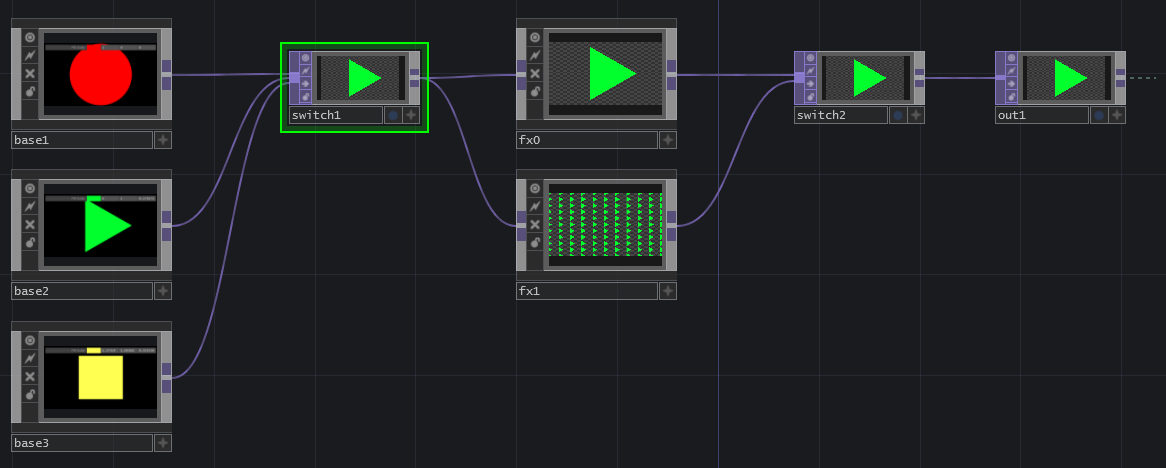
\includegraphics[width=\textwidth]{img/structure2.PNG}
	\caption[shortCaption]
	{inside \texttt{/project1/core}}
	\label{fig:insideCore}
\end{figure}


\paragraph*{Post}
Oftentimes we need some simple post fx such as contrast and color correction feature for adjustment on-site.
\paragraph*{Mapping}
Here we might do our mapping for example using \textbf{Cam Schnappr} or \textbf{Kantan Mapper}. Both of these tools can be found in TouchDesigner's Palette.
\paragraph*{Output}
Our output can be a Window \COMP inside of \texttt{project1}. It should contain both our UI and the image we want to send to our projector(s).
\paragraph*{Local}
The \texttt{local} \COMP is a special \COMP. It simply is a Base \COMP that we renamed to \texttt{local}. This in turn makes TouchDesigner look in there for modules and variables. We will have a look at this at a later point, but to put it simply: It allows us to store states, paths and other variables that make our network more manageable.



\section{Designing a self-contained Component, our first Scene}
Let's have a look at an example scene first:

\begin{figure}[H]
	\centering
	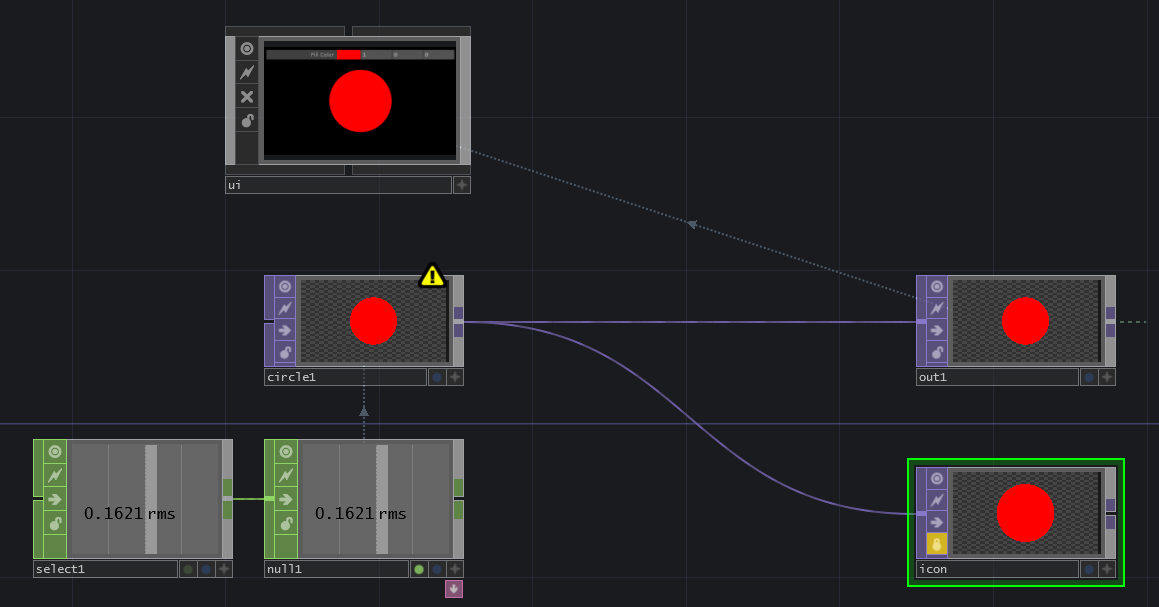
\includegraphics[width=\textwidth]{img/exampleScene.PNG}
	\caption[example scene]
	{example scene, \texttt{/project1/core/scene0}}
	\label{fig:label}
\end{figure}

What we have is some super simplistic imige generator, that is controlled via the RMS of the audio. It's output is sent to the \COMP's output. Also its output was cached at some point into a Null \TOP with the Lock Flag enabled to save the image. The Null \TOP is renamed to \texttt{icon}. This is a convention to later fetch an unanimated preview of what the scene looks like.\\
Also we have a simple GUI in form of a Component \COMP.\\
So let's now see why we chose to layout our exmaple scene this way and what concepts were used here and why.\\

Ideally our scenes are self contained in a sense that we can drag and drop them in any network, they work instantly and we never have to look inside. How can we achieve this? Basically via
\begin{itemize}
	\item \link{https://docs.derivative.ca/index.php?title=Custom\_parameters}{Custom Parameters}
	\item a decent GUI
	\item Sticking to certain standards
	\item enough interconnectivity
	\item Testing. Make sure there are no errors. Because there are errors.
\end{itemize}

We will now have a look at how to build a GUI and how to expose parameters.
An excellent video about how to build components can be found \link{https://www.youtube.com/watch?v=3mgn5SJg1oI}{here}
\subsection{Custom Parameters}
\index{customize component}
\index{custom parameters}
The Custom Parameters feature allows us to add parameters to a Component. We can just right-click on a Component an choose \texttt{Customize Component...} to arrive at the window shown in Figure \ref{fig:customizeComponent}.

\begin{figure}[H]
	\centering
	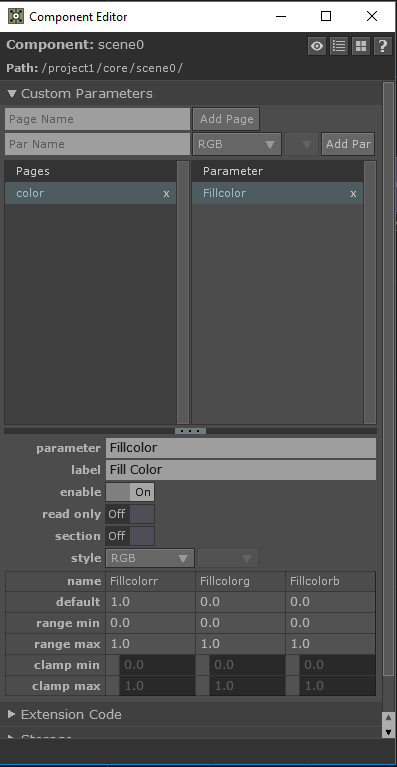
\includegraphics[width=8cm]{img/customizeComponent.PNG}
	\caption[customize component]
	{The Component Editor}
	\label{fig:customizeComponent}
\end{figure}

Here we can add pages and parameters to our component's parameter dialog.\\
Often we will just need to control a parameter of one of our \OPs inside the \COMP directly. We would need to look at the parameter, find the correct type for our custom parameter, and link it to the parameter inside via an expression or CHOP exporting. But there is a nice trick:
We can open the Component Editor, go inside our Component and drag the parameter we want to control to the Parameter list in the Component Editor. This will create a new Parameter with the same name, type and ranges as the original parameter. Also there appears a small pop-up, asking us if we want to automatically create a reference, so the two are linked.

\subsection{Simple GUI}

TouchDesigner is really good for GUI building.
\begin{figure}[H]
	\centering
	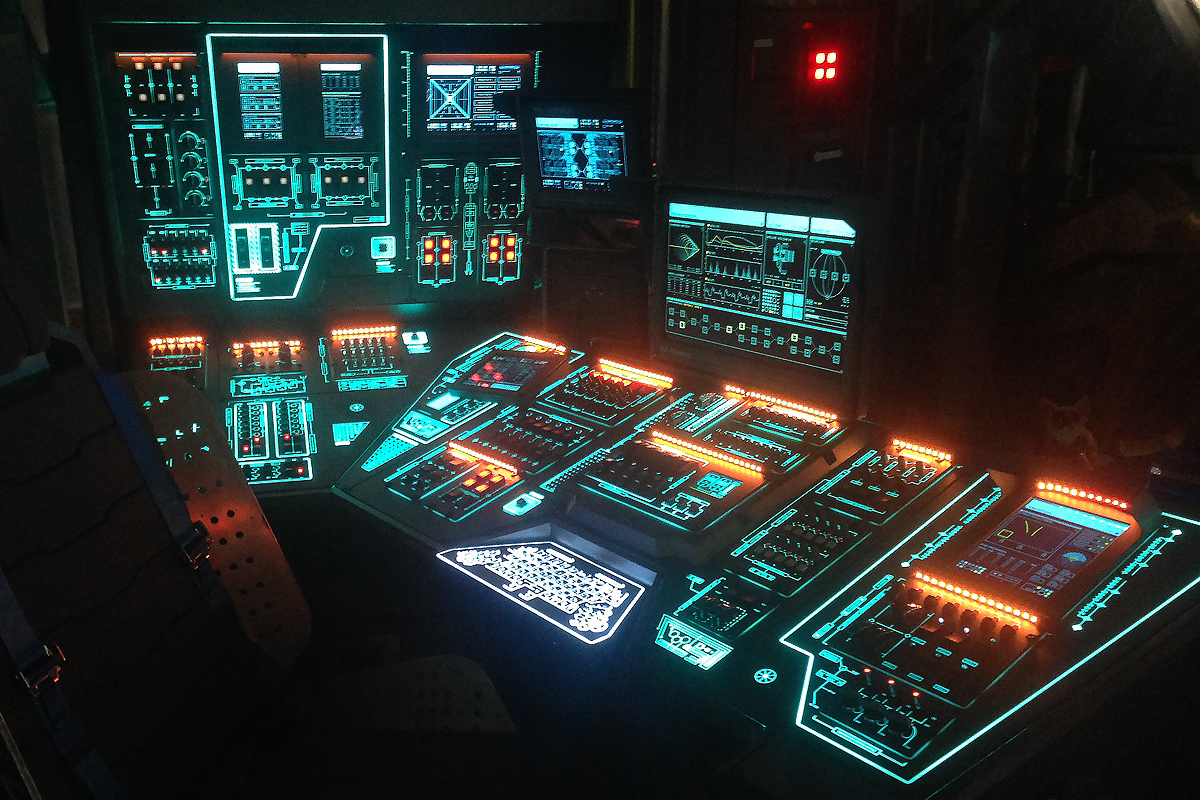
\includegraphics[width=\textwidth]{img/alien.jpg}
	\caption[shortCaption]
	{Image taken from \link{http://derivative.ca/events/2017/AlienCovenant/}{here}. GUIs built in TouchDesigner for the motion picture Alien Covenant}
	\label{fig:label}
\end{figure}


But before getting to complicated, let's look at how we can get the most simplistic GUI going. For our scenes, it would be great if we had a GUI that showed the output of our scene and the important parameters. GUIs are built using one or multiple Container \COMPs.\\
The Container \COMP allows us to align children elements in an orderly hierarchical manner and it generates events and data for mouse interaction such as mouse rollover or click events. \\
Another very handy \COMP is the Parameter \COMP. We can just point it to a parameter of a chosen OP and it displays it.\\
So, to make our example scene display a very simple GUI, we do the following:

\begin{enumerate}
	\item create a Container \COMP
	\item rename it to 'ui'
	\item point its \texttt{background TOP} parameter to out Out \TOP
	\item inside the Container \COMP, create a Parameter \COMP.
	\item adjust the Parameter \COMP to point to important parameters.
	\item in the \texttt{OP Viewer} parameter of our \texttt{scene0} Base \COMP, write \texttt{./ui}, so the scene displays its ui
\end{enumerate}





\subsection{Connections without Patch Cords, the Select OPs}

\begin{figure}[H]
	\centering
	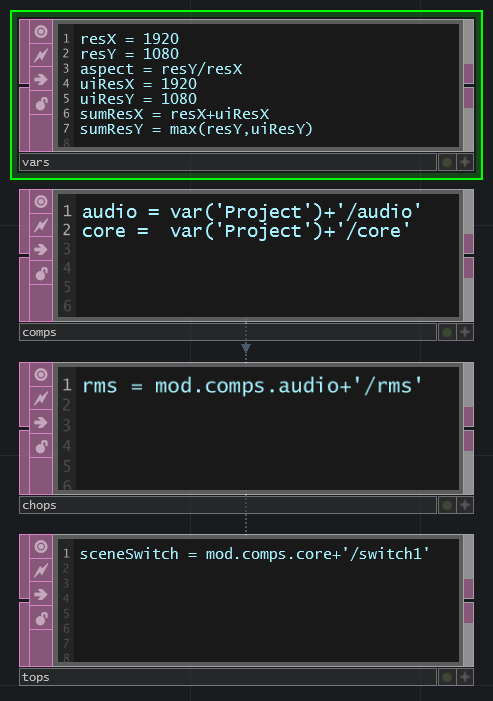
\includegraphics[width=8cm]{img/localModules.PNG}
	\caption[shortCaption]
	{CAPTION MISSING}
	\label{fig:label}
\end{figure}




\subsection{Configuring TD after Install} % (fold)
\label{sub:config}
There are not a lot of things that have to be configured after a fresh install of TD. One of the things that are highly recommended to be adjusted is the text editor\index{text editor}. Sometimes, we write actual text-code inside TouchDesigner, be it \textbf{python}, \textbf{GLSL}, \textbf{TScript}, or another language. We can write this code inside TD itself, but we can also use an external text editor, such as Sublime Text or Notepad+, which provides syntax highlighting, auto-completion and more.\\
In order to conveniently use such an external editor, we just need to go to TD's preferences and specify the path to the external editor.

% to set an \textbf{Environment Variable}. In Windows, there is an application for setting those, the easiest way to access this application is to just search it in the start menu, it's called \textit{Umgebungsvariablen Für dieses Konto bearbeiten} or \textit{Environment Variables}.\\
% Here, a variable called \verb|TOUCH_EDITOR| should be created and it's value should be set to the path to your favorite text editor.\\
After that, anytime we right-click on a \DAT and choose \textit{Edit contents} or press \keystroke{ctrl}+\keystroke{e}, our text editor opens, we can edit the file, save it and will have edited that \DAT.



\subsection{Scripting} % (fold)
\label{sub:scripting}
important helper functions:\\
\begin{lstlisting}
	dir(object) #get attributes of the object
	help(object) #call help on object
\end{lstlisting}

\subsubsection{Referencing \OPs} % (fold)
\label{ssub:referencing}
\OPs and their contents can be referenced in an absolute or relative way. Also, it makes sense to save paths inside variable\index{variable}, as we will see in \ref{ssub:Modules}. to reference a Null \CHOP at \verb|/project1/null1| for example, we can use the expression:
\begin{lstlisting}
	op('/project1/null1')
\end{lstlisting}
We can access the first channel in that Null \CHOP just by issuing \verb|op('/project1/null1')[0]|. Also, a \CHOP's channels may be accessed by their name, so if we had a \CHOP with a channel named \verb|tx| at the same location, we can use \verb|op('/project1/null1')['tx']|. Both of these expressions are useful for animating parameters, and are an alternative to \textbf{CHOP exporting}(see \ref{sub:CHOPs}).

\begin{framed}
	What should I use, \CHOP exporting or python references?
	Python expressions and references tend to be cleaner and more readable.
	\CHOP exporting is faster performance-wise. The team at derivative is constantly working to make python expressions compile to native C code in the backround so simple expresions and references are basically already as fast as \CHOP exporting. \\
	So, if in a certain project, performance is a very critical issue, one should still stick to \CHOP exporting. Otherwise, python expressions are preferable due to readability and overall handyness.
\end{framed}

\subsubsection{Variables} % (fold)
\label{ssub:variables}

In TouchDesigner, there are a number of variable types \footnote{\href{http://www.derivative.ca/wiki088/index.php?title=Variables}{Variables on the TouchDesigner Wiki}}. Within scripts, variables may be defined in a standard pythonic way, such as \verb|a = 5|. For variables that may be accessed throughout a network, \textbf{component variables} are the most useful ones, although
there are a couple of options to get a variable-like behavior\footnote{Other options, that might be more useful depending on the situation are: Referencing a
Null \CHOP, extensions, the storage system, modules containing variables and more}, without defining an actual variable.\\
Variables in TD should not be used for processes that require them to be written very often, such as driving an animation at 60 FPS with a variable. A (time sliced) \CHOP channel makes more sense in such situations. Think of variables rather for purposes of storing application resolution, setting and getting the state of state machines, or similar \glqq{}semi-static\grqq{} values.\\

Component variables in TD are bound to a \COMP. They can be bound to the \textbf{root Component}, but may live in any component. There are many ways to get the value of a variable, as well as setting it. In order to create a variable called \verb|varName|
with the value \verb|5| in the component \verb|/project1| we can execute the command:
\begin{lstlisting}
	op('/project1').setVar('varName', 5)
\end{lstlisting}

This will create a Base \COMP: \verb|/project1/local|. The \verb|local| \COMP is a special \COMP that is automatically referenced in certain situations, such as retrieving a variable or module. We could have created a Base \COMP and renamed it to \verb|local| manually too. Inside this \COMP, our variables are stored via \DATs.\\

 \missingImage \\

For defining variables that can be retrieved everywhere in a network, we typically define a component Variable that is attached to the root component (at \verb|/|). In order to do so, we can execute the command:
\begin{lstlisting}
	root.setVar('varName', 5)
\end{lstlisting}
This will store our new variable inside \verb|/local|. We can now get the value of \verb|varName| by evaluating
\begin{lstlisting}
	var('varName')
\end{lstlisting}
in a parameter or by using an Evaluate \DAT for example, but also simply in the \textbf{Text Port}.


We can override Variables inside specific \COMPs. Let's assume we made a complex network, and we use two root Component variables to set the resolution for all \TOPs in the network. This is good practice, since it makes it easy to change the resolution quickly and globally. But maybe we have some subprocess that is also quite complex and which needs a different resolution. We could make new variables. But what if we could just override the global ones inside just this subprocess? Well, we can, we just need to redefine the variables inside that specific \COMP.\\

Assume our complex subprocess is a base \COMP at \verb|/project1/sub|. We can just define:
\begin{lstlisting}
	root.setVar('resXY', [1280, 720])
	op('/project1/sub').setVar('resXY', [256, 256])
\end{lstlisting}
This way, everywhere in our network, \verb|resXY| will evaluate to the list \verb|[1280, 720]|, but everywhere inside \verb|/project1/sub| it will evaluate to \verb|[256, 256]|.

% subsubsection component_variables (end)
\subsubsection{Modules} % (fold)
\label{ssub:Modules}
\index{Module}Modules are a way to organize variables, functions, classes. Any Text \DAT can hold a module.
let's assume we made a Text \DAT at \verb|/project1/myTools|. In there, we wrote:
\begin{lstlisting}
	x = 5
	def multiplyByTwo(inp):
		return inp*2.
\end{lstlisting}
\testThis


We can now use this Text \DAT as a module. In order to do so, we have couple of options. One would be to use it in another script inside another Text \DAT. For example:
\begin{lstlisting}
	import myTools
	print (myTools.multiplyByTwo(5))
\end{lstlisting}

Another and maybe more common way would be to use it in a parameter, by the MOD (module on demand) class. If our module is inside the search Path (so in the same \COMP for example, or, as we see in a moment, inside \verb|local|) we can use the expression:
\begin{lstlisting}
	mod.myTools.multiplyByTwo(5)
\end{lstlisting}

For information on how to reference a module, and for information about how to import it as efficiently as possible, look \link{http://www.derivative.ca/wiki088/index.php?title=MOD\_Class}{here}

